\chapter{Preliminary Work}\label{C:preliminary}

\section{Problem Formalisation}
A typical Web service composition scenario is that of an online book shopping system, as shown in Figure \ref{fig:compositionExample}. The objective of this system, constructed using existing Web services, is to allow a customer to purchase a book offering different methods of payment according to their account balance. Namely, if the customer has enough money to pay for the selected book, then they would like to pay for it in full; otherwise, they would like to pay for it in instalments. The idea is to construct this system in a fully automated manner, meaning that the services to be used, the connections between these services, and the overall flow of the system are determined automatically. When requesting the creation of a system with the desired functionality, the composition task provided consists of the overall inputs required by the system (e.g. book title, author, customer information), conditional constraints (e.g. the customer's account balance is less than the price of the chosen book), and the potential outputs produced by the system (e.g. a receipt, if the customer paid in full, or an initial bill, if the customer is paying in instalments).

\begin{figure}
\centerline{
\fbox{
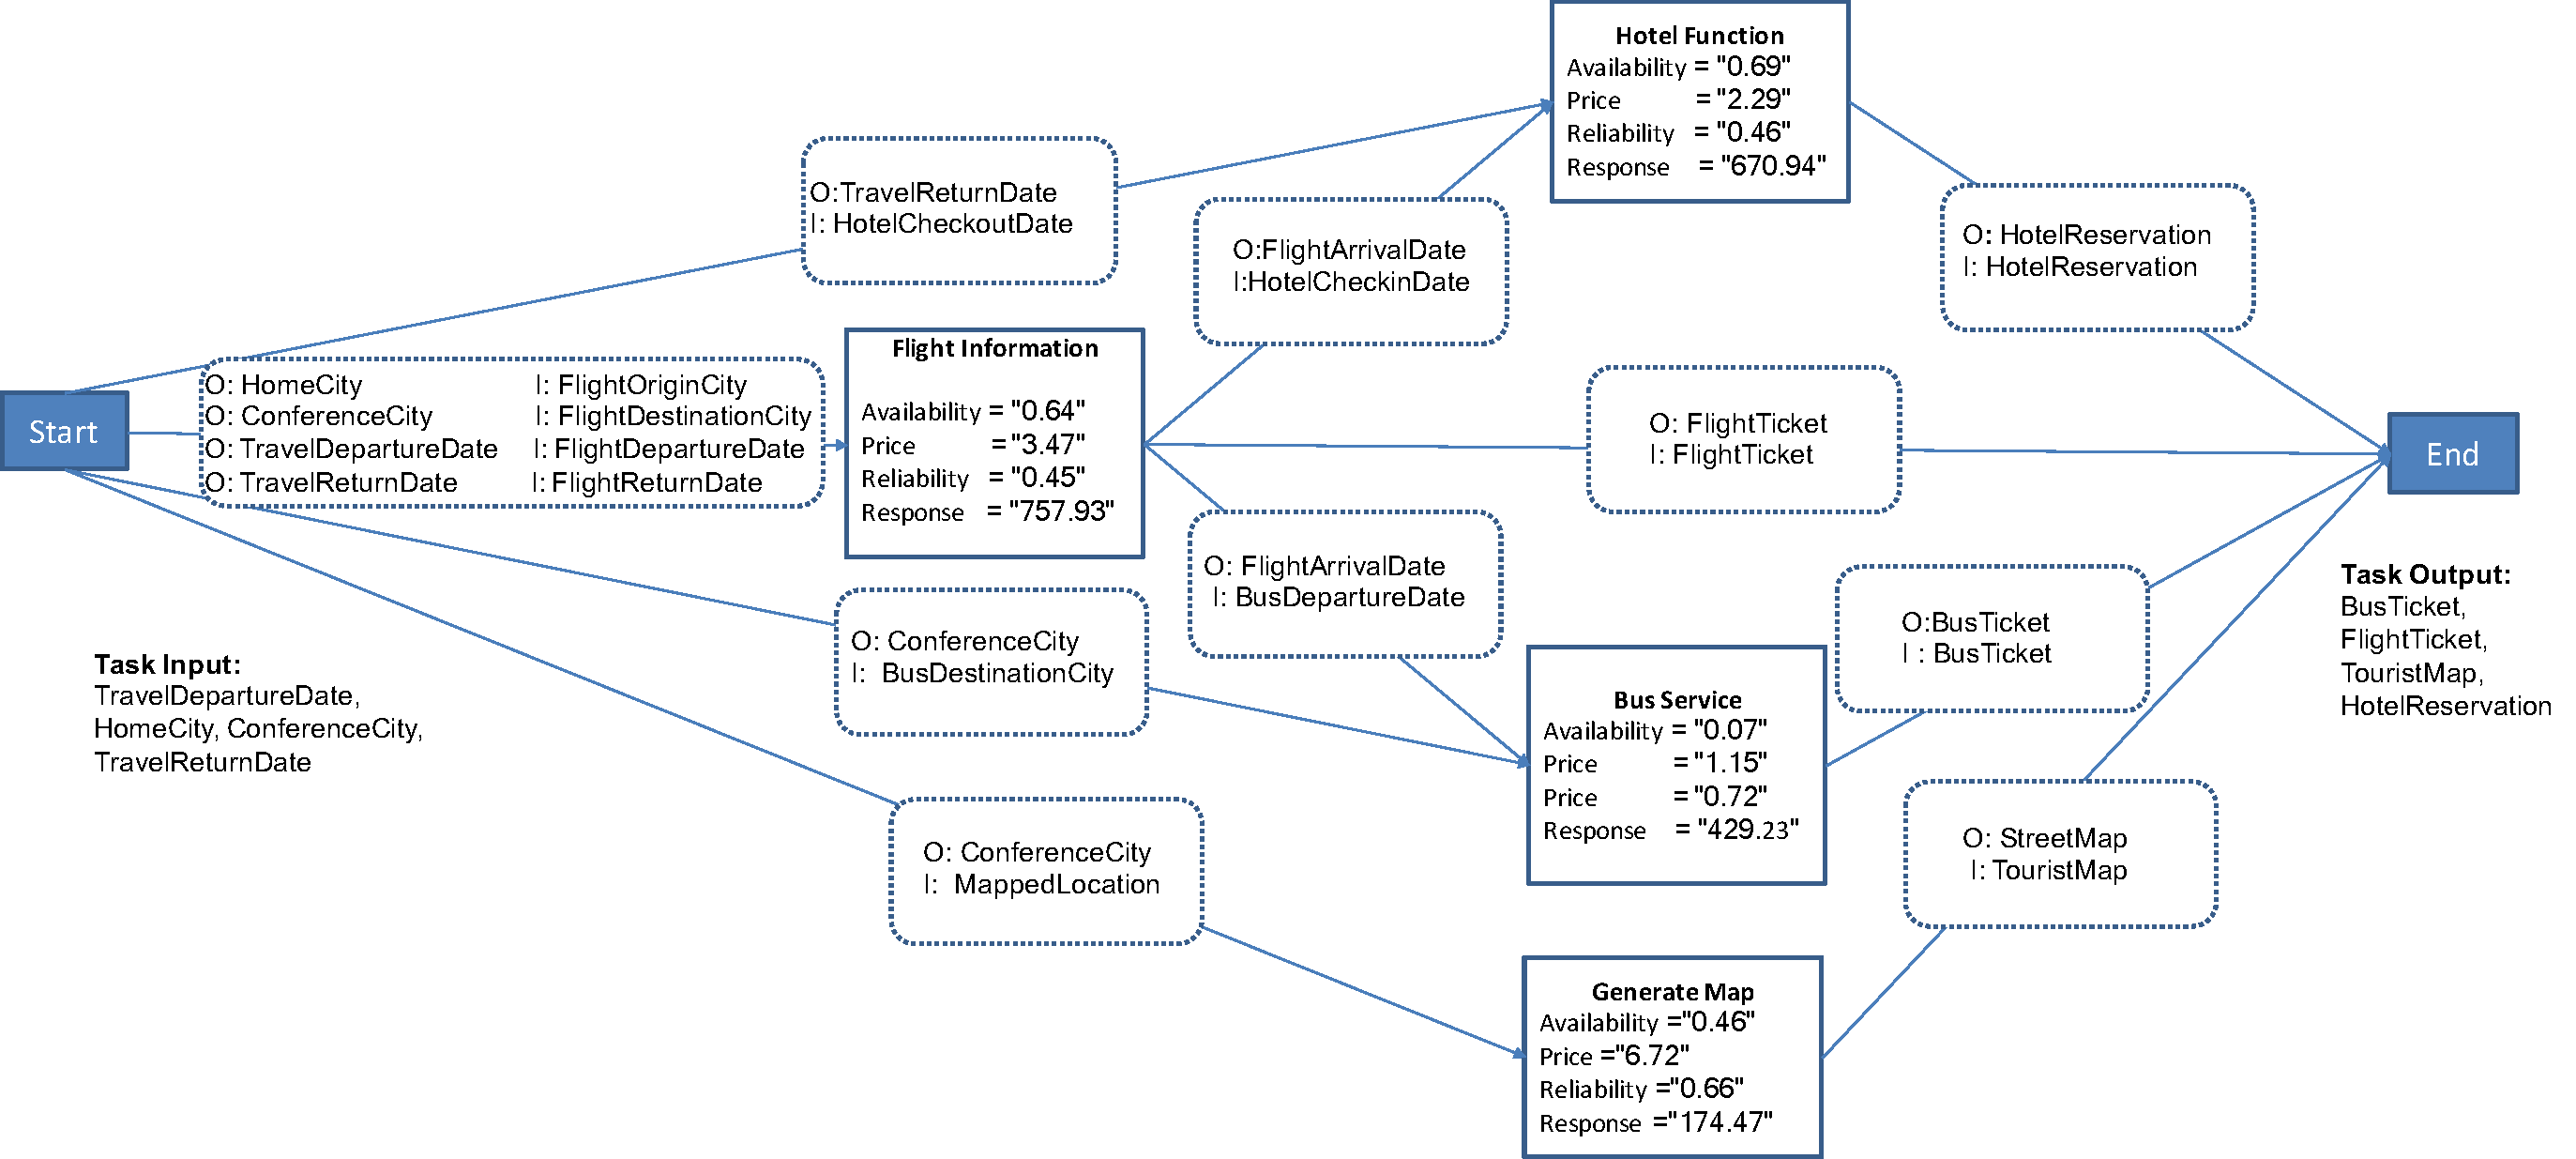
\includegraphics[width=6cm]{motivation.pdf}}}
\caption{A Web composition for an online book shopping system.}
\label{fig:compositionExample}
\end{figure}

More formally, a Web service composition that includes branching can be thought of as a reachability problem where, given a composition input set $I$, a group of services is assembled in order to produce multiple composition output sets $O_1$ to $O_m$, each output being dependent on a sequence of branching conditions $C_1$ to $C_n$ that leads to that outcome. Users often expect these services to be optimised according to their quality, giving higher weights to reflect the priority of quality attributes. Based on this understanding, a \textit{composition task} can be represented as a tuple $T = (P, W)$. $P$ is a collection of paths from the provided input $I$, going through some conditions $C$ to reach one of required output possibilities $O_i$, essentially forming a tree $P = \{\langle I,C,O_i\rangle\}$, and \textit{W} is the set of priority weights for each Quality of Service (QoS) attribute. A \textit{Web service} is a tuple $S_x = (I_x, O_x, Q_x)$, where $I_x$ is the set of inputs that must be provided in order to execute the service, $O_x$ is the set of outputs produced by the service after execution, and $Q_x$ are the service's QoS attributes. Finally, a \textit{Web service composition} is a minimal set of paths where all services appearing in a path are sequentially linked, and where interleaved conditional nodes are allowed. Thus, it can be described as $WSC = \{\langle I,(S,C_x)\star,S,O_i\rangle\}$. The inputs of all services in the sequences $S$ are fully satisfied, if all paths in the composition are considered, and the same is true for the various $O$ possibilities. A property of the paths in $WSC$ is that if all services are removed from a path $a \in WSC$, then its shortened version corresponds to a path in $P$ (i.e. $a_{short} \in P$).

\section{Language Constructs and QoS}

In addition to the functional aspects of Web service composition, the goodness of the services included in a solution also plays a part in the creation of a composite system. This non-functional set of attributes is known as Quality of Service (QoS) \cite{menasce2002qos}, and it measures characteristics that are desirable in a service from a customer's point of view. In this work, four QoS attributes are considered \cite{yu2013adaptive}: Time (T), which measures the response time of a service once it has been invoked, Cost (C), which specifies the financial cost of using a given service, Availability (A), which measures the likelihood of a service being available at invocation time, and Reliability (R), which is the likelihood of a service responding appropriately when invoked.
The existing languages for Web service composition (e.g. BPEL4WS \cite{wohed2003analysis}) use certain constructs to control the flow of the resulting systems with regards to input satisfaction. However, in addition to this functional aspect, they also influence the QoS properties of a composition. The following constructs are considered in this work:

\begin{itemize}
\item\textit{Sequence construct:} In a sequence construct services are chained sequentially, so that the outputs of a preceding service are used to satisfy the inputs of a subsequent service, as shown in Figure \ref{fig:sequence}. The total cost and time of this construct are calculated by adding the values of its individual services, and the total availability and reliability by multiplying them.
\item\textit{Parallel construct:} In a parallel construct services are executed in parallel, so their inputs are independently fulfilled and their outputs are independently produced, as shown in Figure \ref{fig:parallel}. The availability, reliability and cost are calculated the same way as they are in the sequence construct, and the total time is determined by identifying the service with the longest execution time. 
\item\textit{Choice construct:} In a choice construct only one service path is executed, depending on whether the value of its associated conditional constraint is met at runtime. This is shown in Figure \ref{fig:conditional}. In this construct, all overall QoS attributes are calculated as a weighted sum of the services from each individual path, where each weight corresponds to probability of that path being chosen during runtime. These weights add up to 1. 
\end{itemize}

\begin{figure}
\centerline{
\fbox{
\begin{tabular}{p{0.5\linewidth}}
\space\hfill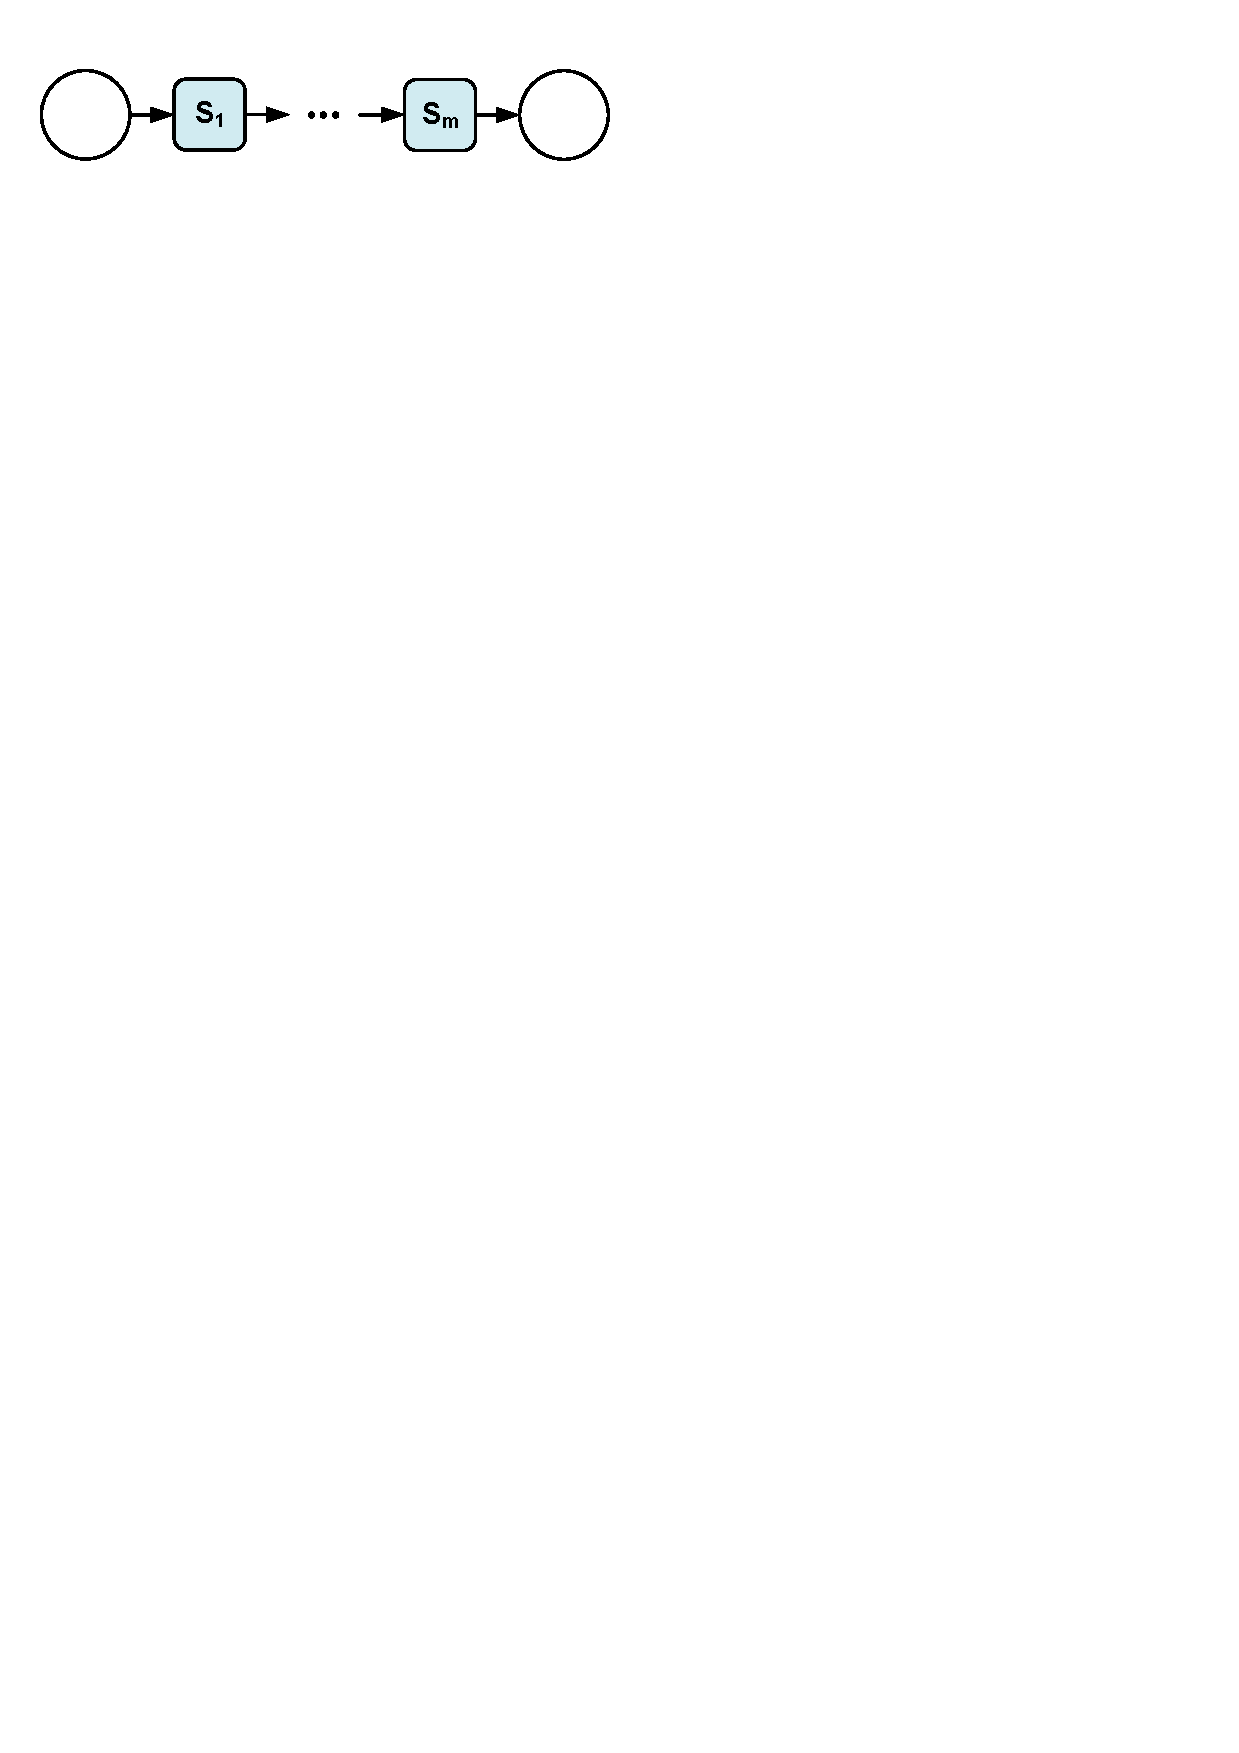
\includegraphics[width=1.4in]{sequence.pdf}\hfill\space\\[0.2cm]
$T=\frac{\sum\limits^m_{n=1}t_n}{m}$ \hfill $C=\frac{\sum\limits^m_{n=1}c_n}{m}$ \hfill
$A=\prod\limits^m_{n=1}a_n$\\
\space\hfill $R=\prod\limits^m_{n=1}r_n$\hfill\space\\[0.2cm]
\end{tabular}}}
\caption{Sequence construct and calculation of its QoS properties.}
\label{fig:sequence}
\vspace{0.3cm}

\centerline{
\fbox{
\begin{tabular}{p{0.5\linewidth}}
\space\hfill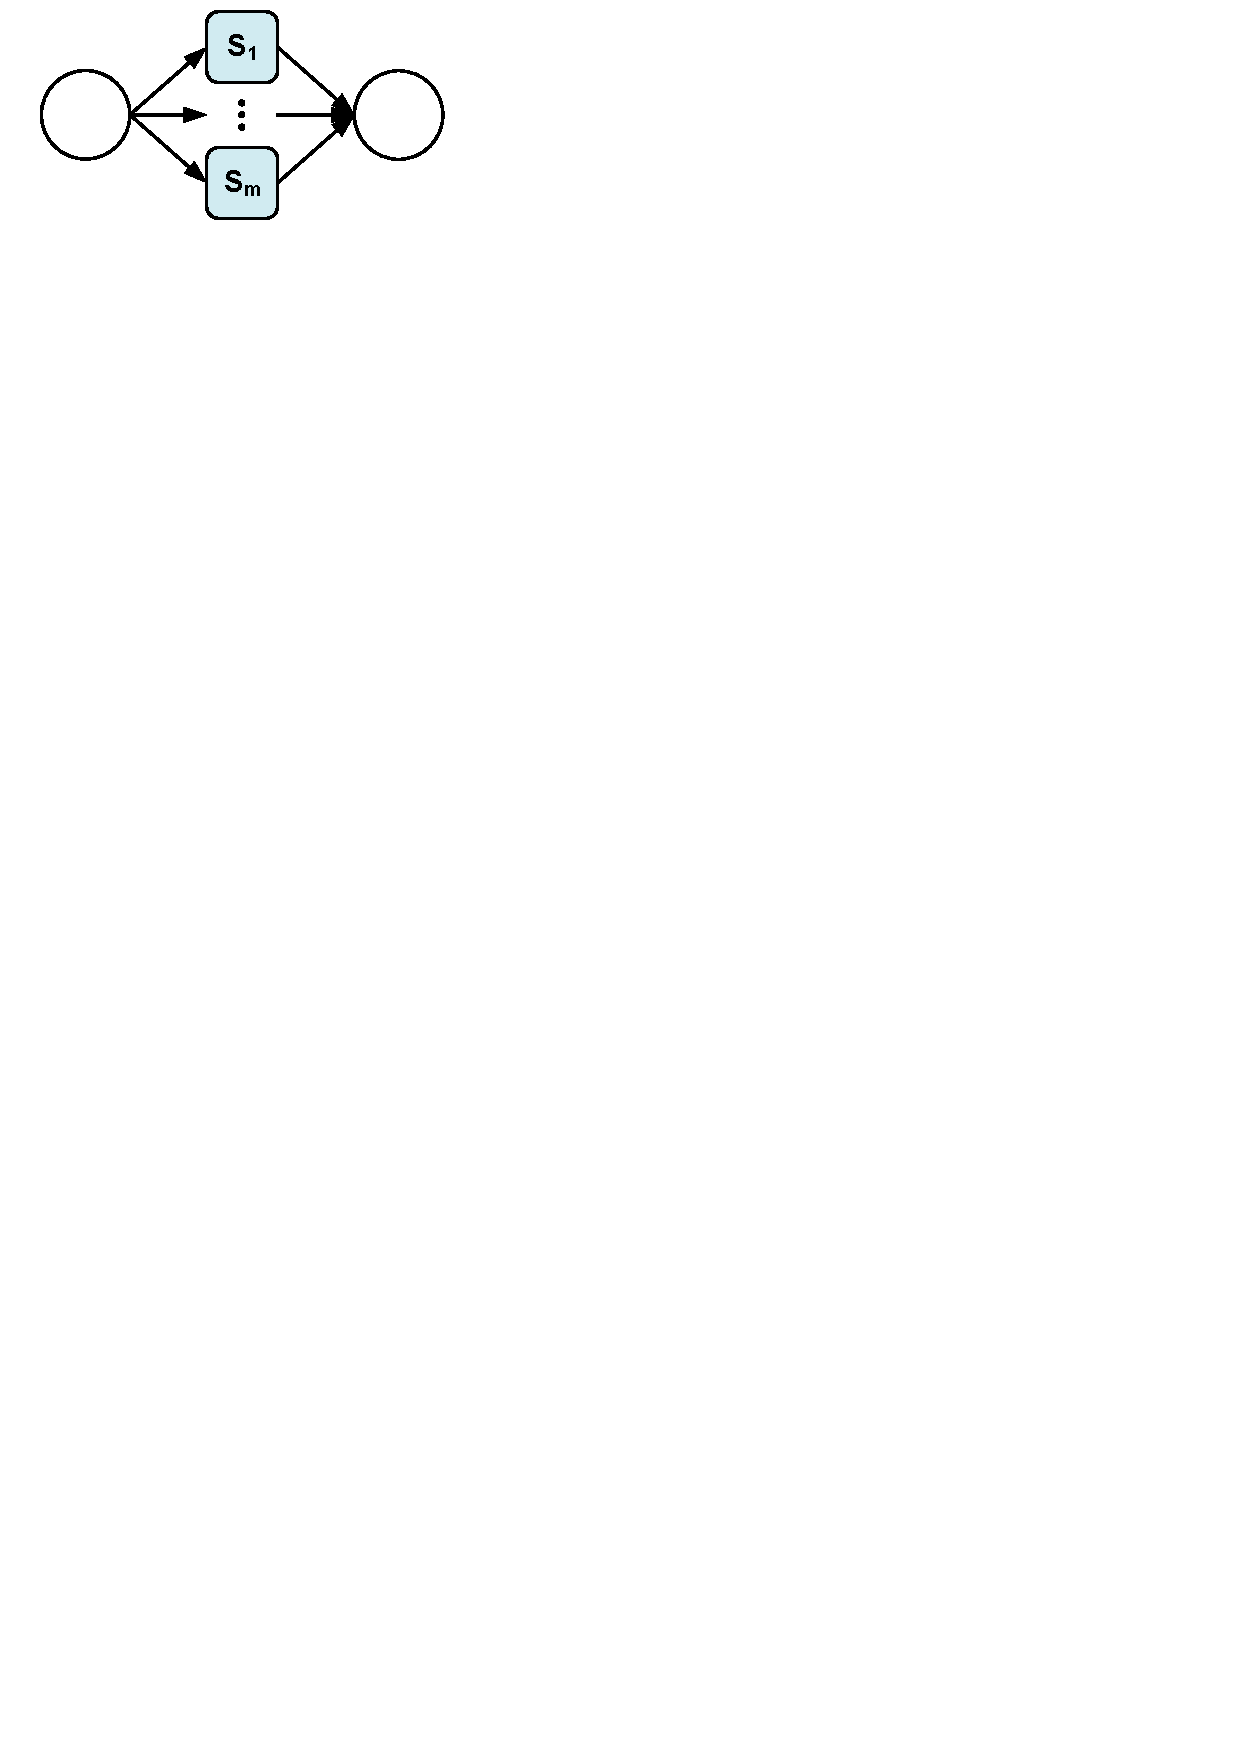
\includegraphics[width=1in]{parallel.pdf}\hfill\space\\[0.2cm]
\space\hfill$T=MAX\{t_n|n\in\{1,\ldots,m\}\}$\hfill\space\\[0.2cm]
$C=\frac{\sum\limits^m_{n=1}c_n}{m}$ \hfill $A=\prod\limits^m_{n=1}a_n$ \hfill
$R=\prod\limits^m_{n=1}r_n$
\end{tabular}}}
\caption{Parallel construct and calculation of its QoS properties.}
\label{fig:parallel}
\vspace{0.3cm}

\centerline{
\fbox{
\begin{tabular}{p{0.5\linewidth}}
\space\hfill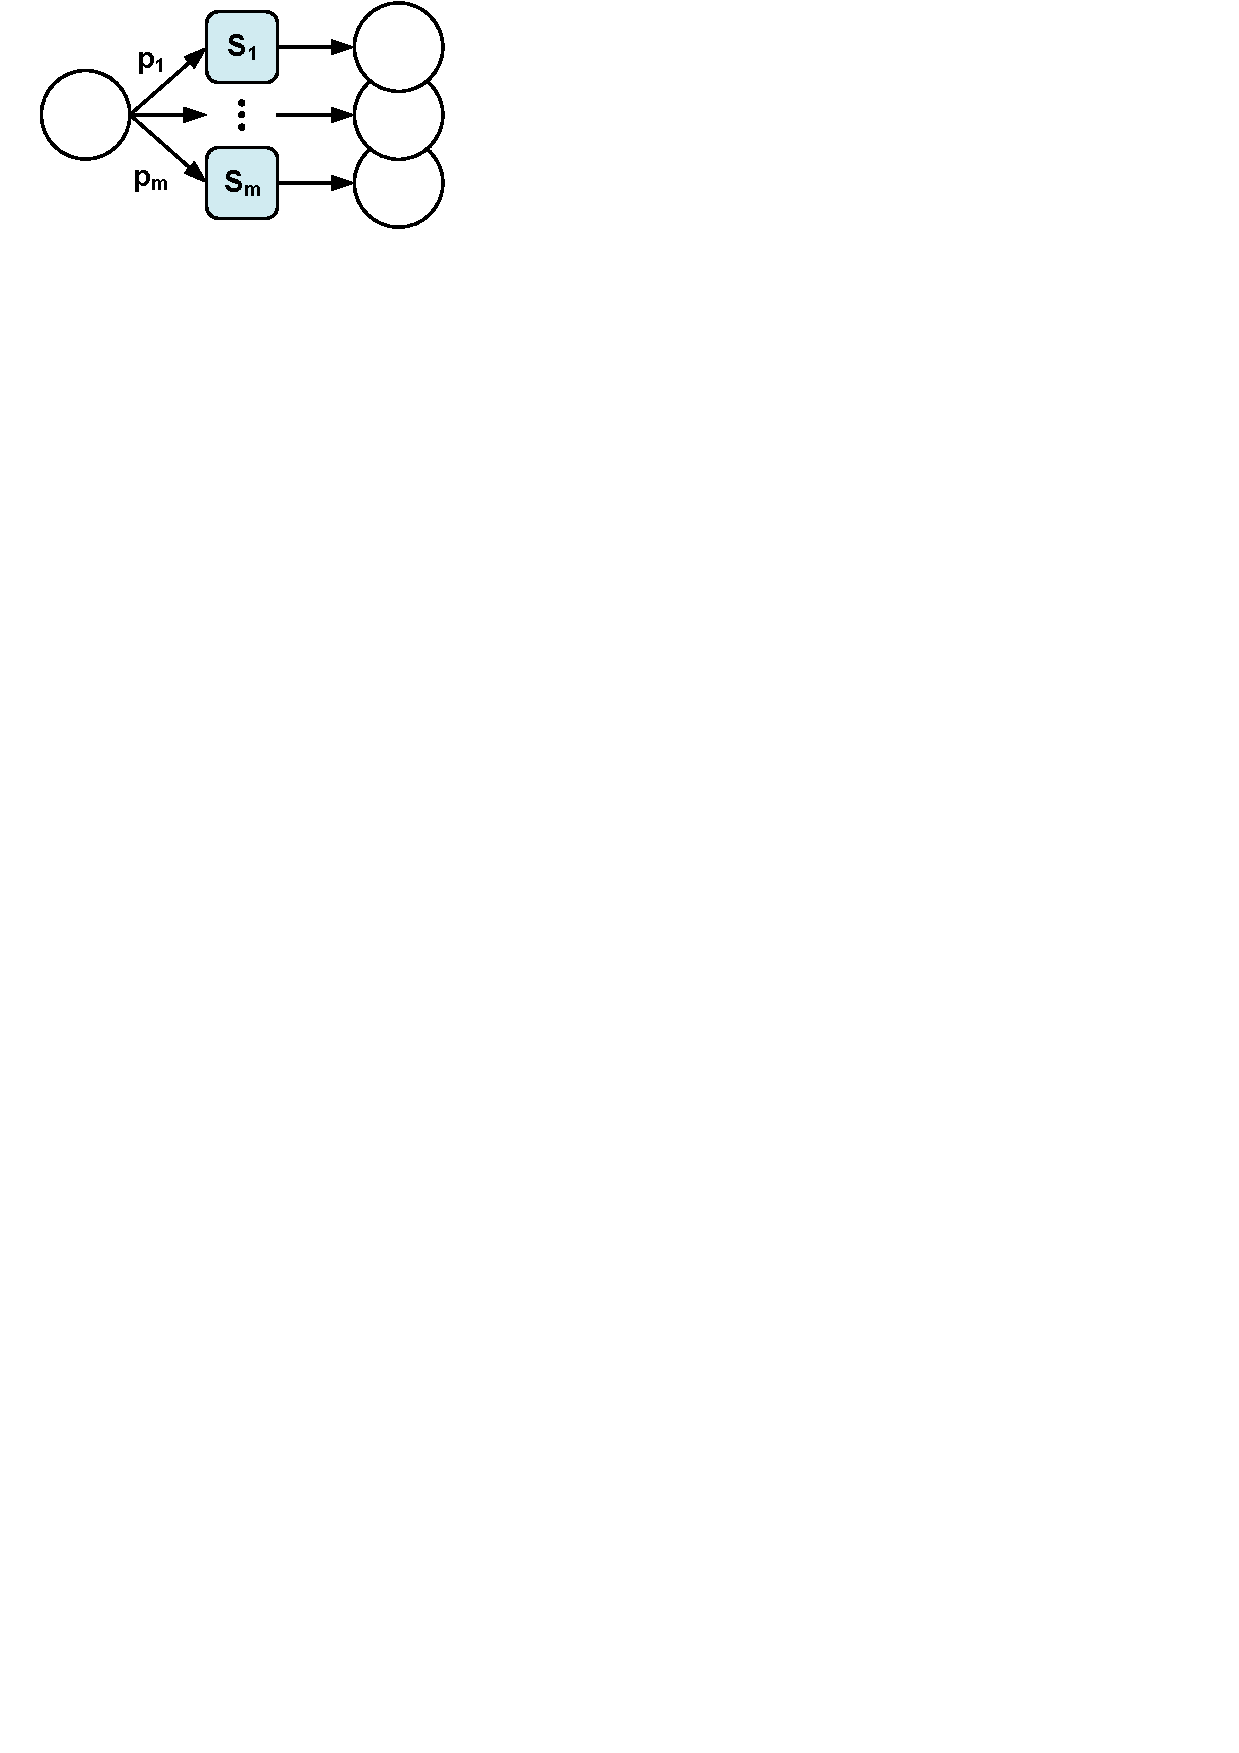
\includegraphics[width=1in]{conditional.pdf}\hfill\space\\[0.2cm]
$T=\sum\limits^m_{n=1}p_{n} t_{n}$ \hfill $C=\sum\limits^m_{n=1}p_{n} c_{n}$\hfill
$A=\sum\limits^m_{n=1}p_{n} a_{n}$\\
\space\hfill$R=\sum\limits^m_{n=1}p_{n} r_{n}$\hfill\space\\[0.2cm]
\end{tabular}}}
\caption{Choice construct and calculation of its QoS properties.}
\label{fig:conditional}
\end{figure}

\section{Fitness Function}
The fitness function is used for optimising solutions according to their overall Quality of Service (QoS), and was based on the function shown in \cite{sawczuk2015gp}. This function measures the overall quality of a composition candidate by performing a weighted sum of the overall QoS attributes of a given candidate:

\begin{equation}
 fitness_i = w_1A_i + w_2R_i + w_3(1 - T_i) + w_4(1 - C_i)
\end{equation}

where $\sum_{i=1}^4{w_i} = 1$ \\

This function produces values in the range [0,1], where a fitness of 1 means the best possible quality, and a fitness of 0 means the worst. Because this is a maximising function, the Time $T$ and cost $C$ are offset by 1 in the formula, so that higher scores correspond to better qualities for these attributes as well. The overall quality attributes $A$, $R$, $T$, and $C$ of a composition are calculated according to formulae shown in Figures \ref{fig:sequence}, \ref{fig:parallel}, and \ref{fig:conditional}, and these values are then normalised to fit within the [0,1] range, according to Formulae \ref{availNormalise}, \ref{reliaNormalise}, \ref{timeNormalise}, and \ref{costNormalise}. These formulae are inspired by the work in \cite{ma2015hybrid}, and normalise the original overall composition values ($A_{orig}$, $R_{orig}$, $T_{orig}$, $C_{orig}$) by using the overall minimum and maximum values for each quality attribute over the entire service repository. In the formulae for calculating $T_i$ and $C_i$ the maximum values are multiplied by the total number $n$ of services in the repository, thus creating an upper bound for the normalisation. This is because a composition including all available candidate services would have the worst possible time and cost attributes.

\begin{equation}
A_i = \begin{cases}
     \frac{A_{orig} - A_{min}}{A_{max} - A_{min}}, & \text{ if }A_{max} - A_{min} \neq 0.\\
     1 & \mathrm{ otherwise}.
    \end{cases}
 \label{availNormalise}
\end{equation}

\begin{equation}
R_i = \begin{cases}
     \frac{R_{orig} - R_{min}}{R_{max} - R_{min}}, & \text{ if }R_{max} - R_{min} \neq 0.\\
     1 & \mathrm{ otherwise}.
    \end{cases}
 \label{reliaNormalise}
\end{equation}

\begin{equation}
T_i = \begin{cases}
     \frac{T_{orig} - T_{min}}{nT_{max} - T_{min}}, & \text{ if }nT_{max} - T_{min} \neq 0.\\
     0 & \text{ otherwise}.
    \end{cases}
 \label{timeNormalise}
\end{equation}

\begin{equation}
C_i = \begin{cases}
     \frac{C_{orig} - C_{min}}{nC_{max} - C_{min}}, & \text{ if }nC_{max} - C_{min} \neq 0.\\
     0 & \text{ otherwise}.
    \end{cases}
 \label{costNormalise}
\end{equation}

\section{Conditional Tree Representation}

\subsection{Movitation}
\subsection{Proposed Approach}
Our proposed approach employs Genetic Programming to evolve solutions according to their overall Quality of Service, meanwhile maintaining their functional correctness. A candidate solution for a composition is represented as a tree, where the non-terminal nodes represent the composition flow constructs (sequence, parallel, and conditional), and the terminal (leaf) nodes represent the atomic Web services included in the composition. An example of such a tree is shown in Figure \ref{fig:tree}. To calculate the overall QoS of a tree, the formulae in Figures \ref{fig:sequence}, \ref{fig:parallel} and \ref{fig:conditional} are employed, where the children of a current node act as the services used in the calculations. For Figure \ref{fig:tree}, for example, the QoS is first calculated for the sequence nodes directly above the leaves, then for the conditional node, and finally for the root node. This is discussed further in Subsection \ref{fitness}.

\begin{figure}
\centerline{
\fbox{
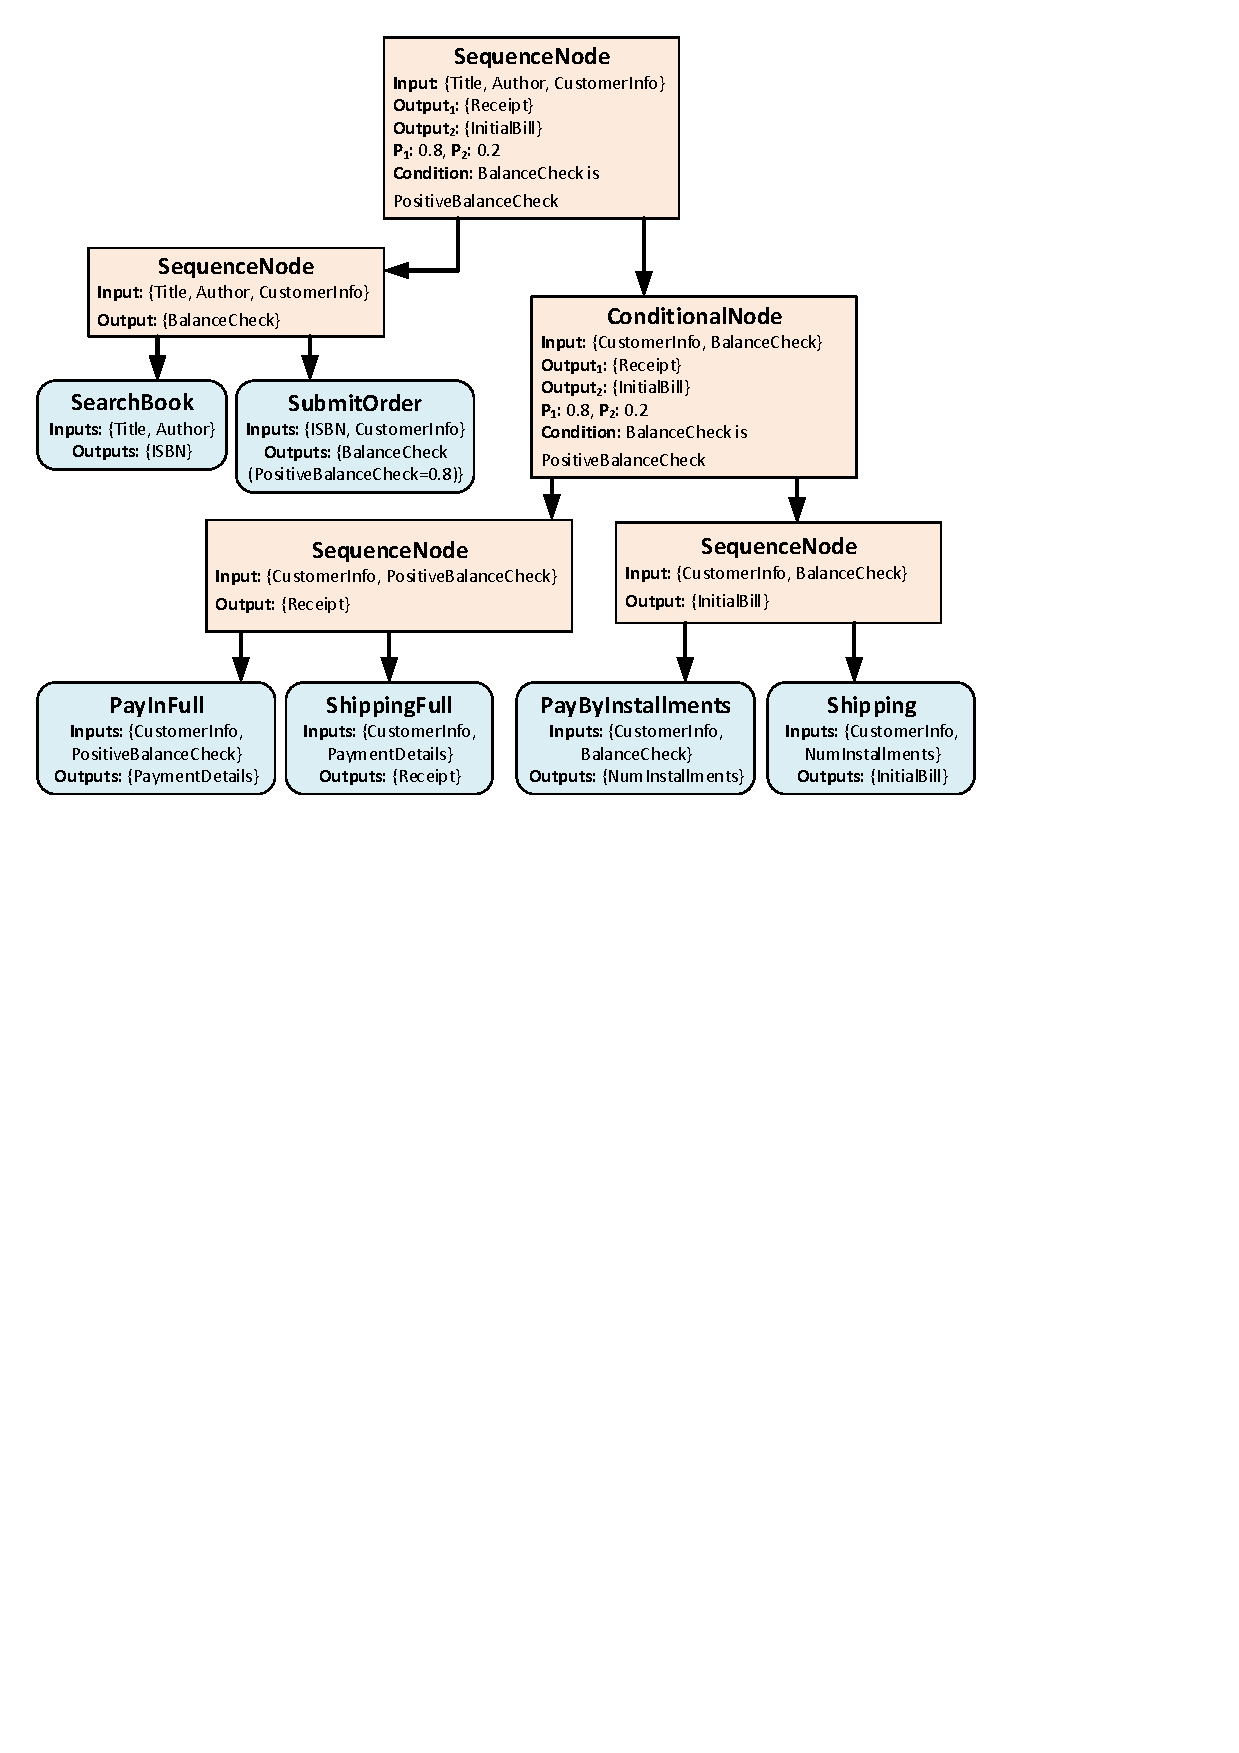
\includegraphics[width=8.4cm]{tree.pdf}
}}
\caption{Example of tree representation for Web service composition.}
\label{fig:tree}
\end{figure}

A population initialisation algorithm similar to the one in \cite{wang2013genetic} is employed, and so are constrained mutation and crossover operations. However, the difference of the current approach in comparison to \cite{wang2013genetic} is that it also considers the case where a user requires a branching constraint to be met, like the one illustrated in Figure \ref{fig:compositionExample}. The presence of branching means that different values are produced by a service at runtime, and these concrete values are subtypes of a statically defined concept. For example, a service that statically outputs a \textit{fruit} concept may output the subtype \textit{banana} at runtime, and thus branching conditions may be defined based on the different kinds of fruits. The relationship between types is held by a taxonomy that encodes the inputs and outputs pertinent to the candidate atomic services employed in the composition. For simplicity, the implementation presented in this work handles branching with two options (if and else), so this scenario will be the focus throughout the following sections.

\subsubsection{Population Initialisation}\label{init}
As opposed to generating a composition candidate purely based on a set of available inputs and another of desired outputs, when handling branching constraints it is also necessary to consider a branching condition. Thus, a composition task with branching must include a set of available inputs, a condition of the is-a kind (e.g. if \textit{banana} $\succeq$ \textit{fruit}), and two sets of outputs, one expected in case the condition is met and the other in case it is not. With this information it is possible to run the initialisation algorithm and create a composition candidate in a graph format, later translated into a tree representation.

\begin{algorithm}
 \setlength\hsize{0.9\linewidth}
 \SetKwInOut{Input}{Input}\SetKwInOut{Output}{Output}
 \SetKwFunction{createGraph}{createGraph}\SetKwFunction{toTree}{toTree}
 \LinesNumbered
 \SetNlSty{}{}{:}
 \Input{$I$, $O_1$, $O_2$, $C$, $P$}
 \Output{candidate tree $T$}
 \eIf{$O_2 \neq \emptyset$}{
  $G_1 \leftarrow \createGraph(I \cup C.if, O_1)$\;
  $G_2 \leftarrow \createGraph(I \cup C.else, O_2)$\;
  $T_1 \leftarrow \toTree(G_1.input)$\;
  $T_2 \leftarrow \toTree(G_2.input)$\;
  $T_3 \leftarrow$ new $ConditionalNode$($C$)\;
  $T_3.leftChild \leftarrow T_1$\;
  $T_3.rightChild \leftarrow T_2$\;
  \eIf{$C \sqsubseteq I$}{
    $T_3.prob \leftarrow P$\;
    \KwRet $T_3$\;
  }{
    $G_4 \leftarrow \createGraph(I, C.else)$\;
    $T_4 \leftarrow \toTree(G_4.input)$\;
    $T_3.prob \leftarrow T_4.final.P$\;
    $T \leftarrow$ new $SequenceNode$()\;
    $T.leftChild \leftarrow T_4$\;
    $T.rightChild \leftarrow T_3$\;
    \KwRet $T$\;
  }
 }{
  $G \leftarrow \createGraph(I, O_1)$\;
  $T \leftarrow \toTree(G.input)$\;
  \KwRet $T$\;
 }
 \vspace{2mm}
 \caption{\footnotesize Generating a new candidate tree or a mutated subtree.}
\label{generation}
\end{algorithm}

Algorithm \ref{generation} is used to create a candidate which may incorporate a branching constraint, though it is also capable of handling unconditional tasks. It requires a
set of inputs $I$, an if-else condition $C$, two sets of outputs $O_1$ (for if-branch) and $O_2$ (for else-branch). The set of probabilities $P$ is only required for a specific case, explained below, and $C$ as well as $O_2$ are not required for tasks without branching. The intuition behind this algorithm is to assemble a candidate tree in parts. Firstly, if the task has in fact two sets of outputs and a condition $C$, then two sub-composition graphs $G_1$ and $G_2$ are generated to represent the if and the else branches, respectively. This generation is performed using the $createGraph$ algorithm proposed in \cite{wang2013genetic}. Subsequently, these graphs are translated to trees $T_1$ and $T_2$ using the $toTree$ procedure proposed in Algorithm \ref{toTree}, and included as children of a $ConditionalNode$ created for condition $C$ (the left child represent the if-branch, and the right child the else-branch).

\begin{algorithm}
 \setlength\hsize{0.9\linewidth}
 \SetKwInOut{Input}{Input}\SetKwInOut{Output}{Output}
 \SetKwFunction{createParallelNode}{createParallelNode}\SetKwFunction{toTree}{toTree}
 \SetKwProg{Procedure}{Procedure}{}{}
 \LinesNumbered
 \SetNlSty{}{}{:}
 \Procedure{\toTree{}}{
 \Input{$N$}
 \Output{tree $T$}
 \uIf{$N$ is leaf}{
  \KwRet $N$\;
  }
  \uElseIf{$N = input$}{
    \eIf{$|N.to| = 1$}{
      $T \leftarrow \toTree(next.to[0])$\;
    }{
      $T \leftarrow \createParallelNode(N.to)$\;
    }
  }
  \uElse{
    $r$\;
    $children \leftarrow N.to - output$\;
    \eIf{$|children| = 1$}{
      $r \leftarrow \toTree(children[0])$\;
    }{
      $r \leftarrow \createParallelNode(children)$\;
    }
    $T \leftarrow$ new $SequenceNode$()\;
    $T.leftChild \leftarrow N$\;
    $T.rightChild \leftarrow r$\;
  }
  \KwRet $T$\;
  }
 \Procedure{\createParallelNode{}}{
 \Input{$children$}
 \Output{tree $T$}
 $T \leftarrow$ new $ParallelNode$()\;
 $subtrees \leftarrow \{\}$\;
 \ForEach{$c$ in $children$}{
    $S \leftarrow\toTree(c)$\;
    $subtrees \leftarrow subtrees \cup \{S\}$\;
 }
 $T.children \leftarrow subtrees$\;
 \KwRet $T$\;
 }
 \vspace{2mm}
 \caption{\footnotesize Converting graph into tree representation.}
\label{toTree}
\end{algorithm} 

Secondly, the algorithm verifies whether the value used for condition $C$ can be met by using the set of inputs $I$. If it can, then the set of probabilities $P$ of each branch being executed is associated to the $ConditionalNode$ and the tree is returned (this assumes that the probabilities for obtaining a specific value for the if condition in $C$ are already known -- typically during mutation). If it cannot, then another sub-composition graph $G_4$ is generated and translated to $T_4$, creating the part of the composition that leads from the available inputs $I$ to the value used in condition $C$. In this case, the probability associated with each branch of the condition is extracted from the last service in $T_4$ (i.e. the service that produces the overall sub-composition output that satisfies the value used in condition $C$), and a $SequenceNode$ is created as the tree root to link this deterministic part of the composition ($T_4$) to the conditional part ($T_3$). Finally, if no condition $C$ and output set $O_2$ are provided, then the candidate is generated purely by using the $createGraph$ and $toTree$ algorithms. 

For reasons of brevity, the $toTree$ procedure shown in Algorithm \ref{toTree} for converting a graph representation of a composition to a tree representation is not explained in detail. Its general idea is the same as the one discussed in \cite{nguyen2005text}, which is to recursively traverse a graph, starting from the start ($input$) node and working towards the end ($output$) node. At each node, the number of outgoing edges determines whether to create a sequential or a parallel construct, and $toTree$ recurses on each of the destination nodes of these outgoing edges. It is important to note that after creating the candidate tree, it must be traversed to determine the input values required to execute each node of the tree, and the output values produced by each node. This information is recorded within each node.

\subsubsection{Mutation and Crossover}\label{mutation}

The crossover operator employed in the evolutionary process swaps any two leaf nodes (i.e. Web services), one from each candidate, provided that these two leaves are functionally equivalent in terms of input and output values but represent different Web services. This particular crossover operation implementation was chosen because it provides an effective mechanism for performing Web service selection, whose objective is to identify the best service to perform a task out of a set of candidates providing the same functionality.
The mutation operator selects a node of the candidate tree at random, and using its input and output information produces a new subtree that may be structurally different yet provides the same functionality. The subtree is generated using Algorithm \ref{generation}, and is used to  replace the originally selected node in the candidate.

\subsubsection{GP Algorithm for Composition}
When applying GP to the service composition problem, each candidate in the population represents a possible candidate solution. The initial population is created as described above, and the fitness of each candidate is evaluated using the fitness function. The fittest individuals are reproduced to the next generation, while other candidates are created in the next generation by applying the mutation and crossover operations to currently promising individuals. This new generation is then evaluated according to the fitness of candidates, and the process is repeated for a fixed number of generations. Lastly, the candidate with the highest fitness in the final population is chosen as the composition solution.

% \section{Graph Representation}
% 
% \subsection{Limitations of Tree Representation}
% \subsection{Proposed Representation}
% \subsection{Experiments}

\section{Conditional Graph Representation}

\subsection{Why Add Branches}

\subsection{Proposed Representation}

The approach proposed in this work is an extension of the GraphEvol technique \cite{sawczuk2015graphevol} to allow for the representation of composite services with multiple execution branches, depending on conditional constraints specified in the composition task. A GraphEvol candidate may look like the representation shown in Figure \ref{fig:compositionExample}, with each block encoded as a graph node, and edges flowing from the input (start) towards the output (end) nodes. However, nodes with multiple children and/or multiple parents can also be included when necessary, meaning that Directed Acyclic Graphs (DAGs) are the basis of this representation. Algorithm \ref{graphEvolSteps} describes the general procedure followed by GraphEvol, and the following subsections explain the ways in which this basic technique was extended to allow for conditional branching.

\begin{algorithm}
 \setlength\hsize{0.9\linewidth}
 \SetKwInOut{Input}{Input}\SetKwInOut{Output}{Output}
 \let\oldnl\nl% Store \nl in \oldnl
\newcommand{\nonl}{\renewcommand{\nl}{\let\nl\oldnl}}
 \LinesNumbered
	\textbf{1.} Initialise the population using the graph building algorithm.\\
	\textbf{2.} Evaluate the fitness of the initialised population.\\
	\nonl \While {max. generations not met}{
	
	\textbf{3.} Select the fittest graph candidates for reproduction.\\
	\textbf{4.} Perform mutation and crossover on the selected candidates, generating offspring.\\
	\textbf{5.} Evaluate the fitness of the new graph individuals.\\
	\textbf{6.} Replace the lowest-fitness individuals in the population with the new graph individuals.\\
	}
 \caption{\footnotesize Steps of the GraphEvol technique \protect\cite{sawczuk2015graphevol}.}
\label{graphEvolSteps}
\end{algorithm}

\subsubsection{Graph building algorithm}
\begin{algorithm}
 \setlength\hsize{0.9\linewidth}
 \SetKwInOut{Input}{Input}\SetKwInOut{Output}{Output}
 \SetKwFunction{connectNode}{connectNode}\SetKwFunction{findCands}{findCands}\SetKwFunction{removeDangling}{removeDangling}\SetKwFunction{buildBranch}{buildBranch}
  \SetKwFunction{buildGraph}{buildGraph}\SetKwFunction{false}{false}\SetKwFunction{null}{null}
 \LinesNumbered
 \SetNlSty{}{}{:}
 %\Input{$InputNode$, $relevant$}
 %\Output{candidate graph $G$}
 
 \SetKwProg{myproc}{Procedure}{}{}
 \myproc{\buildGraph{$InputNode, relevant, candMap$}}{
 $start.outputs \leftarrow \{InputNode.values\}$\;
 $TaskNode \leftarrow InputNode.child$\;
 $G.edges \leftarrow \{\}$\;
 $G.nodes \leftarrow \{\}$\;
 $allInputs \leftarrow \{\}$\;
 $connections \leftarrow \{\}$\;
 \connectNode{$start,connections,G,allInputs,TaskNode$}\;
 $allowedAncestors \leftarrow \{start\}$\;
 \eIf{$candMap$ is \null}{
 $candList \leftarrow$ \findCands{$start,allowedAncestors,relevant$}\;
 }{
 $candList \leftarrow \{node | (start,node) \in candMap\}$\;
 }
 \buildBranch{$TaskNode,candList,connections,allInputs,G,$
 $relevant,allowedAncestors,candMap$}\;
 \removeDangling{$G$}\;
 \KwRet $G$\;
 }
 
 \vspace{2mm}
 \SetKwProg{myproc}{Procedure}{}{}
 \myproc{\connectNode{$n, connections, G, allInputs, TaskNode$}}{
  $n.objective \leftarrow TaskNode$\;
  $G.nodes \leftarrow G.nodes \cup \{n\}$\;
  $G.edges \leftarrow G.edges \cup connections$\;
  \eIf{$TaskNode$ is $ConditionNode$}{
    \eIf{$|n.outputs| > 1$}{
      \KwRet $((TaskNode.general \sqsubseteq n.outputs.general \wedge TaskNode.specific \sqsubseteq n.outputs.specific), n)$\;
    }{
      \KwRet $($\false$,n)$\;
    }
  }{
     \KwRet $(TaskNode.outputs \sqsubseteq allInputs, n)$\;
  }
}
 \caption{\footnotesize Procedures for building a new candidate graph and for connecting a particular node to the graph \protect\cite{sawczuk2015graphevol}.}
\label{generation}
\end{algorithm}

As with the fundamental GraphEvol technique, a graph-building algorithm is used to initialise the population of candidates so that the connections between the different atomic services included in a composition are correct. In this work, however, this algorithm is extended to create solutions with one input but multiple outputs, depending on the branching conditions specified. This extended version is shown in Algorithm \ref{generation}.

Candidates are created using the $buildGraph$ procedure. This procedure requires $InputNode$, which is the root of the composition's task tree, a list of $relevant$ candidate services from the service repository, and optionally a $candMap$. The $candMap$ is used for the crossover procedure only, so it will be discussed later. Given these inputs, the algorithm proceeds to connect nodes to the graph, one at a time, until a complete solution is found. As explained earlier, the resulting composition will have several independent branches, thus the recursive procedure $buildBranch$ has been created to handle each part of the composition. After connecting the $start$ node to the graph, we execute $buildBranch$ providing the first task it should achieve (i.e. $TaskNode$, which initially will be a conditional branching node), a list of candidates $candList$ that contains services that are executable/reachable using the $start$ node outputs, the partially built graph $G$, and other relevant data structures. Once the $buildBranch$ procedure has finished executing, the graph $G$ will be completed. The algorithm used for construction creates graphs from the $start$ node to the $end$ nodes in order to prevent cycles from forming, but this may lead to \textit{dangling} nodes, which are nodes that do not have any outgoing edges despite not being $end$ nodes. These are redundant parts of the solution, and thus they must be removed once $G$ is built. Finally, the creation of the new candidate graph is finished.

Algorithm \ref{generation} also describes the $connectNode$ procedure, used for adding a node to an existing graph. In addition to adding the given node $n$ to $G$, and connecting it using the edges provided in the $connections$ list, this procedure also checks if the current $TaskNode$ objective has been reached. If the $TaskNode$ represents a conditional node, we check that we are now capable of producing both the  values required by the \textit{if} case and by the \textit{else} case when using the service we have just connected. On the other hand, if the $TaskNode$ represents the $end$ of a branch, we check that the list $allInputs$ of potential inputs contain all values necessary to satisfy the inputs fo the $end$ node.

\begin{algorithm}
 \setlength\hsize{0.9\linewidth}
 \SetKwFunction{connectNode}{connectNode}\SetKwFunction{findCands}{findCands}\SetKwFunction{removeDangling}{removeDangling}\SetKwFunction{buildBranch}{buildBranch}
 \SetKwFunction{false}{false} \SetKwFunction{true}{true}\SetKwFunction{null}{null}\SetKwFunction{connectTaskNode}{connectTaskNode}
 \LinesNumbered
 \SetNlSty{}{}{:}

 \SetKwProg{myproc}{Procedure}{}{}
 \myproc{\buildBranch{$TaskNode,candList,allInputs,G,$\\
 $relevant,allowedAncestors,candMap$}}{
  $goalReached \leftarrow$ \false\;
  $connResult$\;
  \While{$\lnot goalReached$}{
  $found \leftarrow$ \false\;
   \ForEach{$cand \in candList$}{
    $connections \leftarrow \{\}$\;
    $ancestors \leftarrow \{x.outputs | x \in G \wedge x \in allowedAncestors\}$\;
    \If{$cand.inputs \sqsubseteq ancestors$}{
      $connections \leftarrow connections \cup \{x \leftarrow minimal(ancestors)\}$\;
      $found \leftarrow$ \true\;
    }
   
   \If{$found$}{
   	$connResult \leftarrow$ \connectNode{$cand,connections,G,allInputs,TaskNode$}\;
   	$goalReached \leftarrow connResult[0]$\;
   	$allowedAncestors \leftarrow allowedAncestors \cup \{cand\}$\;
   	\eIf{$candMap$ is \null}{
   	$candList \leftarrow candList \cup$ \findCands{$cand,allowedAncestors,relevant$}\;
   	}{
   	$candList \leftarrow candList \cup \{node | (cand,node) \in candMap\}$\;
   	}
   	break\;
   }
   }
     $candList \leftarrow candList - \{cand\}$
  }
  \connectTaskNode{$TaskNode,connResult,G,allowedAncestors,$
  $candList,candMap$}\;
  }
 \caption{\footnotesize Indirectly recursive procedure for building one of the branches of the new candidate graph.}
\label{recursiveAlgo}
\end{algorithm}

Algorithm \ref{recursiveAlgo} shows the $buildBranch$ procedure, which recursively creates the branched Web service composition. Given a $TaskNode$, this procedure repeatedly adds 
services to the graph $G$, until the $TaskNode$ goal has been reached. More specifically, nodes from the $candList$ are considered for addition. A candidate $cand$ is randomly chosen from $candList$, and it is connected to the graph (using the $connectNode$) procedure if all of its inputs can be fulfilled by the $ancestor$ outputs (i.e. the outputs of nodes already present in that particular execution branch). The set of services in $connections$, which are used to connect $cand$ to $G$, is a minimal set, meaning that the output of these services fulfils all the inputs of $cand$, but if any connection is removed from the set that is no longer the case. After each $cand$ service is connected to $G$, the $candList$ is updated to contain any services that have now become executable due to the outputs of $cand$, and to exclude $cand$. Once the $TaskNode$ goal has been reached, the $connectTaskNode$ procedure is called to finish the construction of that branch, either by connecting an $end$ node to it or by further splitting the branch according to a new $TaskNode$ condition. In case of the latter, $connectTaskNode$ will invoke the $buildBranch$ procedure again.

\begin{algorithm}
 \setlength\hsize{0.9\linewidth}
 \SetKwFunction{connectNode}{connectNode}\SetKwFunction{findCands}{findCands}\SetKwFunction{removeDangling}{removeDangling}\SetKwFunction{buildBranch}{buildBranch}
 \SetKwFunction{false}{false} \SetKwFunction{true}{true}\SetKwFunction{null}{null}\SetKwFunction{connectTaskNode}{connectTaskNode}
 \LinesNumbered
 \SetNlSty{}{}{:}

 \SetKwProg{myproc}{Procedure}{}{}
 \myproc{\connectTaskNode{$TaskNode,connResult,G,$
 $allowedAncestors,candList,candMap$}}{
  \eIf{$TaskNode$ is $ConditionalNode$}{
  	$TaskGoal.probs \leftarrow connResult[1].probs$\;
  	$G.nodes \leftarrow G.nodes \cup \{TaskNode\}$\;
  	$G.edges \leftarrow G.edges \cup \{connResult[1] \rightarrow TaskNode\}$\;
  	$allowedAncestors \leftarrow allowedAncestors \cup \{TaskNode\}$\;
  	$connections \leftarrow \{\}$\;
  	\eIf{$candMap$ is \null}{
	  $candList \leftarrow candList \cup$ \findCands{$TaskNode, allowedAncestors, relevant$}\;
  	}{
  	$candList \leftarrow candList \cup \{node | (TaskNode,node) \in candMap\}$\;
  	}
  	$allInputs \leftarrow \{\}$\;
  	$ifChild \leftarrow TaskNode.ifChild$\;
  	\If{$ifChild$ is $OutputNode$}{
	   $allInputs \leftarrow \{x.outputs | x \in allowedAncestors\}$\;  	
  	}
  	\buildBranch{$ifChild, candList, allInputs, G, relevant,$
  	$allowedAncestors,candMap$}\;
  	$elseChild \leftarrow TaskNode.elseChild$\;
  	\If{$elseChild$ is $OutputNode$}{
  		$allInputs \leftarrow \{x.outputs | x \in allowedAncestors\}$\;
  	}
  	\buildBranch{$elseChild, candList, allInputs, G, relevant,$
  	$allowedAncestors,candMap$}\;
  }{
  $ancestors \leftarrow \{x.outputs | x in G \wedge x \in allowedAncestors\}$\;
  $connections \leftarrow \{x \rightarrow TaskNode\ | x \in minimal(ancestors)\}$\;
  $G.nodes \leftarrow G.nodes \cup \{TaskNode\}$\;
  $G.edges \leftarrow G.edges \cup connections$\;
  }
  }
 \caption{\footnotesize Procedure for finishing construction of a branch, splitting it further in case another
 condition exists.}
\label{taskAlgo}
\end{algorithm}

As previously explained, Algorithm \ref{taskAlgo} is responsible for finishing the construction of a given execution branch, according to one of two scenarios. In the first scenario, the $TaskNode$ reached is a conditional node, meaning that the branch will be further split into an \textit{if-and-else} structure. In this case, the $TaskNode$ is added to $G$, connected through the previously added service in $connResult[1]$ (i.e. the service that fulfilled the outputs required for the condition to be checked). Whenever a branching node is added, probability values must be associated with each path, indicating the likelihood of that path being executed. Since the branching occurs based on the values produced by  
$connResult[1]$, the probabilities of producing these different output possibilities are copied from this service. Then, the $buildBranch$ procedure is invoked twice more, once for the $if$ branch and once for the $else$ branch, providing the appropriate children of $TaskNode$ to the next construction stages. In the second scenario, the $TaskNode$ reached is an output node, meaning that the branch leads to an $end$ node without any further splitting. In this case, the $TaskNode$ is simply connected to $G$, using a minimal set of services already in the graph which produce all the outputs required by this $end$ node.

\subsubsection{Mutation and Crossover}

\begin{algorithm}
 \setlength\hsize{0.9\linewidth}
 \SetKwFunction{connectNode}{connectNode}\SetKwFunction{findCands}{findCands}\SetKwFunction{removeDangling}{removeDangling}\SetKwFunction{buildBranch}{buildBranch}
 \SetKwFunction{false}{false} \SetKwFunction{true}{true}\SetKwFunction{null}{null}\SetKwFunction{connectTaskNode}{connectTaskNode}\SetKwFunction{mutation}{mutation}
 \SetKwFunction{crossover}{crossover}\SetKwFunction{selectNode}{selectNode} \SetKwFunction{removeNodes}{removeNodes}
 \LinesNumbered
 \SetNlSty{}{}{:}

 \SetKwProg{myproc}{Procedure}{}{}
 \myproc{\mutation{$G, InputNode, relevant$}}{
 $n \leftarrow$ \selectNode{$G$}\;
 \eIf{$n$ is $start$}{
  \KwRet \buildGraph{$InputNode, relevant,$ \null}\;
 }{
  $TaskNode \leftarrow n.objective$\;
  \removeNodes{$n$}\;
  $allInputs \leftarrow \{\}$\;
  $candList \leftarrow \{\}$\;
  $allowedAncestors \leftarrow \{\}$\;
  \ForEach{$node \in G.nodes$}{
    $allowedAncestors \leftarrow allowedAncestors \cup \{node\}$\;
  }
  \ForEach{$node \in G.nodes$}{
    $candList \leftarrow candList \cup$ \findCands{$node, allowedAncestors, relevant$}\;
  }
  \If{$TaskNode$ is $OutputNode$}{
    $allInputs \leftarrow \{x.outputs | x \in allowedAncestors\}$\;
  }
  \KwRet \buildBranch{$TaskNode, candList, allInputs, G, relevant,$
  $allowedAncestors,$\null}\;
 }
 }
 
  \myproc{\crossover{$G_1, G_2, InputNode, relevant$}}{
  $candMap \leftarrow \{(x,y) | x \rightarrow y \in G_1.edges\}$\;
  $candMap \leftarrow candMap \cup \{(x,y) | x \rightarrow y \in G_2.edges\}$\;
  \KwRet \buildGraph{$InputNode, relevant, candMap$}\;
  }
 
 \caption{\footnotesize Procedures for performing mutation and crossover on graph candidates \protect\cite{sawczuk2015graphevol}.}
\label{operatorsAlgo}
\end{algorithm}

The procedures for performing the mutation and crossover operations are shown in Algorithm \ref{operatorsAlgo}. The general idea behind the $mutation$ procedure is to modify a part of the original graph $G$, but maintain the rest of the graph unchanged. In order to do so, a node $n$ is initially selected as the mutation point, provided that it is not an $end$ or a $condition$ node. If this node is the $start$ node, an entirely new candidate graph is constructed; otherwise, all nodes whose input satisfaction depends upon node $n$ are removed from $G$, and so are any subsequent splits of that branch. The construction of this partially-built graph is then finished by invoking the $buildBranch$ procedure and providing the original $TaskNode$ ($n$'s objective) and appropriate data structures to it. The $allowedAncestors$, the $candList$, and $allInputs$ are calculated based on the remaining nodes of $G$. The mutation operator was designed in this way so that it allows for variations of the original candidate, at the same time maintaining the correctness of the connections between services (nodes) in the graph.

In the case of $crossover$, the general idea is to reuse connection patterns from two existing candidates $G_1$ and $G_2$ in order to create a new child candidate that combines elements from these two parents. In order to do so, the original connections of $G_1$ and $G_2$ are abstracted into a map called $candMap$. This map can be queried to determine all the connections (from both parents) that can be made starting from a given node $x$, e.g. $x$ connects to $y_1$, $y_2$, and $y_3$ in $G_1$ and $G_2$. After having assembled this map, the $buildGraph$ procedure is invoked to create a child candidate. The difference is that the addition of candidates to the $candList$ is done by querying the $candMap$ to determine which services could be reached from the current node according to the connection patterns in the original parents. One of the advantages of this crossover implementation is that it allows for a flexible operation that reuses connection information from both parents. Additionally, this operation can be executed using the already existing graph-building algorithm with minimal changes.

\section{Experiments}
